\documentclass[a4paper,11pt]{article}

% Kodovani (cestiny) v dokumentu: utf-8
%\usepackage[cp1250]{inputenc}	% Omezena stredoevropska kodova stranka, pouze MSW.
\usepackage[utf8]{inputenc}	% Doporucujeme pouzivat UTF-8 (unicode).

\usepackage[margin=2cm]{geometry}
\newtoks\jmenopraktika \newtoks\jmeno \newtoks\datum
\newtoks\obor \newtoks\skupina \newtoks\rocnik \newtoks\semestr
\newtoks\cisloulohy \newtoks\jmenoulohy
\newtoks\tlak \newtoks\teplota \newtoks\vlhkost

\jmenopraktika={Fyzikální praktikum 1}
\jmeno={Lukáš Lejdar}
\datum={27. února 2023}
\obor={F}
\skupina={Út 16:00}

\cisloulohy={4}
\jmenoulohy={Měření gravitační konstanty a tíhového zrychlení}

\tlak={101{,}35}
\teplota={21,1}
\vlhkost={47,7}

%%%%%%%%%%% Uzitecne balicky:
\usepackage[czech]{babel}

\usepackage{graphicx}
\usepackage{amsmath}
\usepackage{xspace}
\usepackage{url}
\usepackage{indentfirst}
\usepackage{wrapfig}
\usepackage{xcolor}
\usepackage{caption}

%%%%%% Zamezeni parchantu:
\widowpenalty 10000 \clubpenalty 10000 \displaywidowpenalty 10000
%%%%%% Parametry pro moznost vsazeni vetsiho poctu obrazku na stranku
\setcounter{topnumber}{3}	  % max. pocet floatu nahore (specifikace t)
\setcounter{bottomnumber}{3}	  % max. pocet floatu dole (specifikace b)
\setcounter{totalnumber}{6}	  % max. pocet floatu na strance celkem
\renewcommand\topfraction{0.9}	  % max podil stranky pro floaty nahore
\renewcommand\bottomfraction{0.9} % max podil stranky pro floaty dole
\renewcommand\textfraction{0.1}	  % min podil stranky, ktery musi obsahovat text
\intextsep=8mm \textfloatsep=8mm  %\intextsep pro ulozeni [h] floatu a \textfloatsep pro [b] or [t]

% Tecky za cisly sekci:
\renewcommand{\thesection}{\arabic{section}.}
\renewcommand{\thesubsection}{\thesection\arabic{subsection}.}
% Jednopismenna mezera mezi cislem a nazvem kapitoly:
\makeatletter \def\@seccntformat#1{\csname the#1\endcsname\hspace{1ex}} \makeatother
%
\newcommand{\vsn}[4]{\ensuremath{#1 =} #2(#3)\,#4}
\newcommand{\vrn}[6]{\ensuremath{#1 =} (#2 $\pm$ #3)\,#4 ($p=$ #5\,\%, $\nu=$ #6)}


%%%%%%%%%%%%%%%%%%%%%%%%%%%%%%%%%%%%%%%%%%%%%%%%%%%%%%%%%%%%%%%%%%%%%%%%%%%%%%%
% Zacatek dokumentu
%%%%%%%%%%%%%%%%%%%%%%%%%%%%%%%%%%%%%%%%%%%%%%%%%%%%%%%%%%%%%%%%%%%%%%%%%%%%%%%

\begin{document}

\thispagestyle{empty}

{
\begin{center}
\sf 
{\Large Ústav fyziky a technologií plazmatu Přírodovědecké fakulty Masarykovy univerzity} \\
\bigskip
{\huge \bfseries FYZIKÁLNÍ PRAKTIKUM} \\
\bigskip
{\Large \the\jmenopraktika}
\end{center}

\bigskip

\sf
\noindent
\setlength{\arrayrulewidth}{1pt}
\begin{tabular*}{\textwidth}{@{\extracolsep{\fill}} l l}
\large {\bfseries Zpracoval:}  \the\jmeno & \large  {\bfseries Naměřeno:} \the\datum\\[2mm]
\large  {\bfseries Obor:} \the\obor  \hspace{40mm}  {\bfseries Skupina:} \the\skupina %
&\large {\bfseries Testováno:}\\
\\
\hline
\end{tabular*}
}

\bigskip

{
\sf
\noindent \begin{tabular}{p{4cm} p{0.6\textwidth}}
\Large  Úloha č. {\bfseries \the\cisloulohy:} \par
\smallskip
$T=\the\teplota$~$^\circ$C \par
$p=\the\tlak$~kPa \par
$\varphi=\the\vlhkost$~\%
&\Large \bfseries \the\jmenoulohy  \\[2mm]
\end{tabular}
}

\vskip1cm

\section{Úvod}

V úloze se pokusím změřit gravitační konstantu $G$ Cavendishovou metodou a tíhové zrychlení pomocí reverzního kyvadla.

\section{Teorie}

\subsection{Měření tíhového zrychlení reverzním kyvadlem }

Pro periodu kmitů T fyzikálního kyvadla platí aproximativní vztah

\begin{equation}
T = 2\pi \sqrt{\frac{J}{mgx}},
\end{equation}

\noindent
kde g je tíhové zrychlení, J moment setrvačnosti kyvadla vzhledem k ose otáčení, m jeho hmotnost a x~vzdálenost těžiště kyvadla od osy otáčení. Tíhové zrychlení se dá určit přímo z tohoto vztahu, ale rádi bychom se vyhnuli měření ošemetných veličin jako je moment setrvačnosti. Používá se proto raději tzv. reverzní kyvadlo se dvěma osami otáčení $o_1$ a $o_2$.

\begin{figure}[htpb]
  \centering
  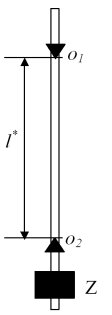
\includegraphics[width=0.12\textwidth]{reverzni_kyvadlo.jpg}
  \caption{Reverzní kyvadlo}
\end{figure}

Označím $x_1$, $x_2$ vzdálenosti těžiště od os $o_1, o_2$.

\begin{align}
  T_1 = 2\pi \sqrt{\frac{J_0+mx_1^2}{mgx_1}}, \quad T_2 = 2\pi \sqrt{\frac{J_0 + mx_2^2}{mgx_2}} 
\end{align}

Pokud zajistíme stejnou periodu kmitů $T_1$=$T_2$, můžeme dosazením $l = x_1 + x_2$, obě T vyjádřit jako

\begin{equation}
T = 2 \pi \sqrt{\frac{l}{g}} 
\end{equation}

\subsection{Měření gravitační konstanty Cavendishovou metodou}

Dvě malé kuličky spojené tyčinkou jsou zavěšené na torzním vlákně a dohromady tak tvoří tlumený harmonický oscilátor: Při zkroucení jeho závěsu o úhel $\varphi$ působí na soustavu vratný silový moment~$M$

\begin{equation}
M(\varphi) = -D\varphi,
\end{equation}

\noindent
kde D je veličina zvaná direkční moment. Po stranách jsou navíc umístěné dvě větší koule působící na oscilátor momentem gravitační síly $M_{\text{grav}}$ jako na obrázku 2. Zanedbáme-li její proměnlivost během torzních kmitů, můžeme z rovnice (4) vyjádřit posun rovnovážné polohy $\varphi_0$

\begin{align}
  \varphi_0 &= \frac{M_{\text{grav}}}{D}.
\end{align}

Při odvozování velikosti momentu gravitačních sil musíme vzít v úvahu, že velká koule působí na obě kuličky, a že momenty těchto sil jsou orientovány proti sobě. Dosazením z Newtonova gravitačního zákona dostaneme

\begin{equation}
  M_{\text{grav}} = 2GMmd \left( \frac{1}{r^2} - \frac{r}{(4d^2+r^2)^{\frac{3}{2}}} \right),
\end{equation}

\noindent
kde G je gravitační konstanta, M hmotnost velké koule a m hmotnost kuličky. 

\begin{figure}[htpb]
  \centering
  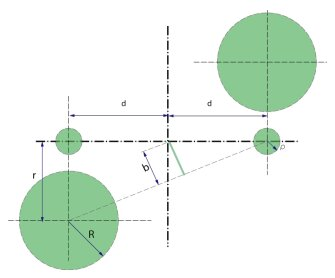
\includegraphics[width=0.52\textwidth]{cavendish_vahy.jpg}
  \caption{Schéma torzních vah Cavendishovy metody při pohledu shora.}
\end{figure}

\newpage

Zbývá najít způsob jak změřit veličinu D. Volné kmity netlumeného torzního kyvadla jsou popsané diferenciální rovnicí

\begin{equation}
J \ddot{\varphi} + D \varphi = M_{\text{grav}},
\end{equation}

\noindent
kde J je moment setrvačnosti kuliček vzhledem k ose otáčení

\begin{equation}
J = 2m ( \frac{2}{5} \rho^2 + d^2).
\end{equation}

Vyřešením rovnice (7) dostaneme

\begin{equation}
\varphi(t) = \varphi_m \sin(\sqrt{\frac{D}{J}}  t  + \psi) + \varphi_0
\end{equation}

\noindent
odkud jde jednoduše spočítat D, pokud zjistíme periodu kmitání.

\section{Postup měření}

\subsection{Měření reverzním kyvadlem}

Pro výpočet potřebuju docílit stejných period kmitání na osách o1 a o2, přičemž jedinou proměnou je posuvné závaží na konci kyvadla. Provedu několik měření period $T_1$ a $T_2$ pro náhodné umístění závaží~x a výsledky vynesu do grafu. Místo kde se křivky pro jednu a druhou osu protnou bude můj první hrubý odhad, který potom budu iterativně malými posuvy zlepšovat.

\subsection{Cavendishova metoda}

V aparatuře je laser namířený na torzní kyvadlo, který se sérií zrcadel projektuje na opačnou stěnu místnosti. Vychýlení kyvadla o úhel $\varphi$ tedy způsobí i vychýlení laseru o ten samý úhel. Aparatura mi zároveň umožňuje obě větší koule zrcadlově vyměnit, tak aby výchylka $\varphi_0$ byla stejná, ale na opačnou stranu. Spustím měření a po uplynutí dostatečně dlouhé doby koule právě takhle vyměním. Výsledná závislost polohy laseru na čase by měla vypadat nějak takto

\begin{figure}[htpb]
  \centering
  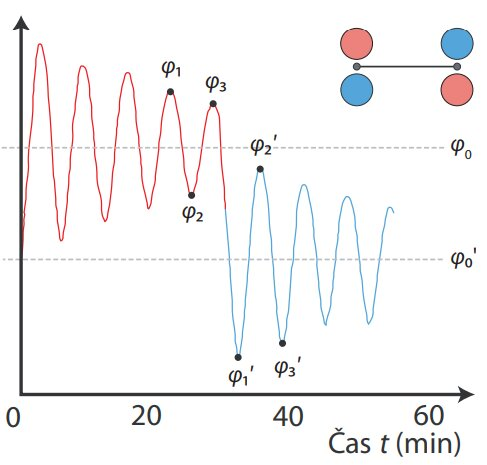
\includegraphics[width=0.48\textwidth]{cavendish_demo_mereni.jpg}
  \caption{Předpokládaná závislost polohy laseru na čase}
\end{figure}

\newpage

Rovnovážnou polohu určím metodou tří kyvů; $\varphi_0 = \frac{1}{2}(\frac{\varphi_1 + \varphi_3}{2} + \varphi_2$) a rovnici (5) přepíšu do této notace jako

\begin{equation}
\varphi_0 - \varphi_0' = 2 \frac{M_{\text{grav}}}{D}.
\end{equation}

Ve skutečnosti ale měřím vzdálenosti na stěně místo úhlů. Platí mezi nimi převodní vztah

\begin{equation}
\varphi_0 - \varphi_0' = 2\arctan(\frac{x_0 - x_0'}{2L}),
\end{equation}

\noindent
kde L je vzdálenost stínítka od oscilátoru.

\section{Výsledky měření}

\subsection{Měření reverzním kyvadlem}
Nejprve jsem provedl několik měření period kmitání na obou osách v závislosti na poloze závaží. Hrubý odhad polohy~$x_0$, zjistím z průniků fitů hodnot.

\begin{figure}[htpb]
  \centering
  % GNUPLOT: LaTeX picture with Postscript
\begingroup
  \makeatletter
  \providecommand\color[2][]{%
    \GenericError{(gnuplot) \space\space\space\@spaces}{%
      Package color not loaded in conjunction with
      terminal option `colourtext'%
    }{See the gnuplot documentation for explanation.%
    }{Either use 'blacktext' in gnuplot or load the package
      color.sty in LaTeX.}%
    \renewcommand\color[2][]{}%
  }%
  \providecommand\includegraphics[2][]{%
    \GenericError{(gnuplot) \space\space\space\@spaces}{%
      Package graphicx or graphics not loaded%
    }{See the gnuplot documentation for explanation.%
    }{The gnuplot epslatex terminal needs graphicx.sty or graphics.sty.}%
    \renewcommand\includegraphics[2][]{}%
  }%
  \providecommand\rotatebox[2]{#2}%
  \@ifundefined{ifGPcolor}{%
    \newif\ifGPcolor
    \GPcolorfalse
  }{}%
  \@ifundefined{ifGPblacktext}{%
    \newif\ifGPblacktext
    \GPblacktexttrue
  }{}%
  % define a \g@addto@macro without @ in the name:
  \let\gplgaddtomacro\g@addto@macro
  % define empty templates for all commands taking text:
  \gdef\gplbacktext{}%
  \gdef\gplfronttext{}%
  \makeatother
  \ifGPblacktext
    % no textcolor at all
    \def\colorrgb#1{}%
    \def\colorgray#1{}%
  \else
    % gray or color?
    \ifGPcolor
      \def\colorrgb#1{\color[rgb]{#1}}%
      \def\colorgray#1{\color[gray]{#1}}%
      \expandafter\def\csname LTw\endcsname{\color{white}}%
      \expandafter\def\csname LTb\endcsname{\color{black}}%
      \expandafter\def\csname LTa\endcsname{\color{black}}%
      \expandafter\def\csname LT0\endcsname{\color[rgb]{1,0,0}}%
      \expandafter\def\csname LT1\endcsname{\color[rgb]{0,1,0}}%
      \expandafter\def\csname LT2\endcsname{\color[rgb]{0,0,1}}%
      \expandafter\def\csname LT3\endcsname{\color[rgb]{1,0,1}}%
      \expandafter\def\csname LT4\endcsname{\color[rgb]{0,1,1}}%
      \expandafter\def\csname LT5\endcsname{\color[rgb]{1,1,0}}%
      \expandafter\def\csname LT6\endcsname{\color[rgb]{0,0,0}}%
      \expandafter\def\csname LT7\endcsname{\color[rgb]{1,0.3,0}}%
      \expandafter\def\csname LT8\endcsname{\color[rgb]{0.5,0.5,0.5}}%
    \else
      % gray
      \def\colorrgb#1{\color{black}}%
      \def\colorgray#1{\color[gray]{#1}}%
      \expandafter\def\csname LTw\endcsname{\color{white}}%
      \expandafter\def\csname LTb\endcsname{\color{black}}%
      \expandafter\def\csname LTa\endcsname{\color{black}}%
      \expandafter\def\csname LT0\endcsname{\color{black}}%
      \expandafter\def\csname LT1\endcsname{\color{black}}%
      \expandafter\def\csname LT2\endcsname{\color{black}}%
      \expandafter\def\csname LT3\endcsname{\color{black}}%
      \expandafter\def\csname LT4\endcsname{\color{black}}%
      \expandafter\def\csname LT5\endcsname{\color{black}}%
      \expandafter\def\csname LT6\endcsname{\color{black}}%
      \expandafter\def\csname LT7\endcsname{\color{black}}%
      \expandafter\def\csname LT8\endcsname{\color{black}}%
    \fi
  \fi
    \setlength{\unitlength}{0.0500bp}%
    \ifx\gptboxheight\undefined%
      \newlength{\gptboxheight}%
      \newlength{\gptboxwidth}%
      \newsavebox{\gptboxtext}%
    \fi%
    \setlength{\fboxrule}{0.5pt}%
    \setlength{\fboxsep}{1pt}%
    \definecolor{tbcol}{rgb}{1,1,1}%
\begin{picture}(8640.00,3888.00)%
    \gplgaddtomacro\gplbacktext{%
      \csname LTb\endcsname%%
      \put(946,253){\makebox(0,0)[r]{\strut{}$0.96$}}%
      \put(946,799){\makebox(0,0)[r]{\strut{}$0.98$}}%
      \put(946,1345){\makebox(0,0)[r]{\strut{}$1$}}%
      \put(946,1892){\makebox(0,0)[r]{\strut{}$1.02$}}%
      \put(946,2438){\makebox(0,0)[r]{\strut{}$1.04$}}%
      \put(946,2984){\makebox(0,0)[r]{\strut{}$1.06$}}%
      \put(946,3530){\makebox(0,0)[r]{\strut{}$1.08$}}%
      \put(1419,-104){\makebox(0,0){\strut{}$70$}}%
      \put(2556,-104){\makebox(0,0){\strut{}$80$}}%
      \put(3694,-104){\makebox(0,0){\strut{}$90$}}%
      \put(4831,-104){\makebox(0,0){\strut{}$100$}}%
      \put(5968,-104){\makebox(0,0){\strut{}$110$}}%
      \put(7106,-104){\makebox(0,0){\strut{}$120$}}%
      \put(8243,-104){\makebox(0,0){\strut{}$130$}}%
    }%
    \gplgaddtomacro\gplfronttext{%
      \csname LTb\endcsname%%
      \put(4109,1077){\makebox(0,0)[l]{\strut{}$x_0$=92.7 $T_0$=1.0}}%
      \csname LTb\endcsname%%
      \put(209,1891){\rotatebox{-270.00}{\makebox(0,0){\strut{}T $\cdot$ 0.5 (s)}}}%
      \put(4660,-434){\makebox(0,0){\strut{}x (mm)}}%
    }%
    \gplbacktext
    \put(0,0){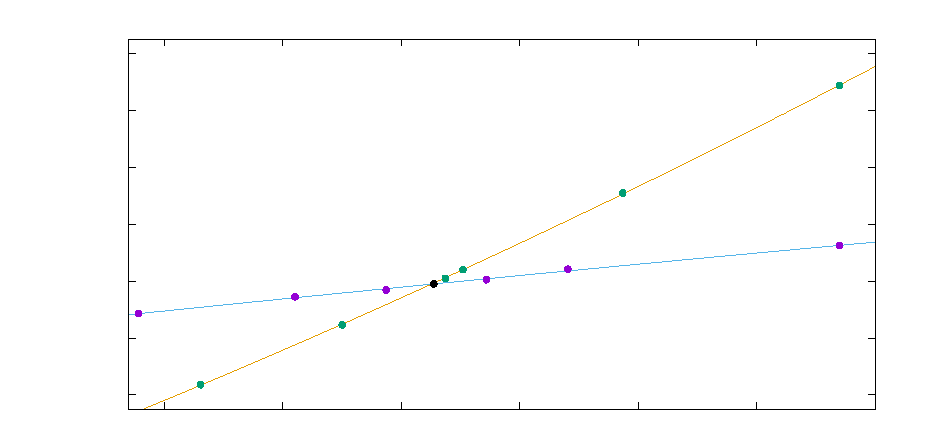
\includegraphics[width={432.00bp},height={194.40bp}]{reverzni_kyvadlo_mereni}}%
    \gplfronttext
  \end{picture}%
\endgroup

  \caption{Závislost doby periody $T$ na poloze závaží pro obě osy}
\end{figure}

Závaží bylo potřeba ještě několikrát nepatrně posunout, než jsem dospěl k nejlepší shodě

\begin{equation}
T_1 = (0.99860 \pm 0.00002)\ s,\ T_2 = (0.99845 \pm 0.00002)\ s,
\end{equation}

Jako výslednou periodu budu považovat průměr hodnot a nejistotu jako jejich rozdíl. Stačí už jenom dosadit vzdálenost os l do vztahu (3) a můžu dopočítat gravitační zrychlení. 

\begin{align}
  T &= (0.99853 \pm 0.0002) \ s \\
  l &= (89.90 \pm 0.03) \text{ cm} \\
  g &= (9.800 \pm 0.004) \text{ ms}^{-2}
\end{align}

\newpage

\subsection{Měření gravitační konstanty Cavendishovou metodou}

\begin{figure}[htpb]
  \centering
  % GNUPLOT: LaTeX picture with Postscript
\begingroup
  \makeatletter
  \providecommand\color[2][]{%
    \GenericError{(gnuplot) \space\space\space\@spaces}{%
      Package color not loaded in conjunction with
      terminal option `colourtext'%
    }{See the gnuplot documentation for explanation.%
    }{Either use 'blacktext' in gnuplot or load the package
      color.sty in LaTeX.}%
    \renewcommand\color[2][]{}%
  }%
  \providecommand\includegraphics[2][]{%
    \GenericError{(gnuplot) \space\space\space\@spaces}{%
      Package graphicx or graphics not loaded%
    }{See the gnuplot documentation for explanation.%
    }{The gnuplot epslatex terminal needs graphicx.sty or graphics.sty.}%
    \renewcommand\includegraphics[2][]{}%
  }%
  \providecommand\rotatebox[2]{#2}%
  \@ifundefined{ifGPcolor}{%
    \newif\ifGPcolor
    \GPcolorfalse
  }{}%
  \@ifundefined{ifGPblacktext}{%
    \newif\ifGPblacktext
    \GPblacktexttrue
  }{}%
  % define a \g@addto@macro without @ in the name:
  \let\gplgaddtomacro\g@addto@macro
  % define empty templates for all commands taking text:
  \gdef\gplbacktext{}%
  \gdef\gplfronttext{}%
  \makeatother
  \ifGPblacktext
    % no textcolor at all
    \def\colorrgb#1{}%
    \def\colorgray#1{}%
  \else
    % gray or color?
    \ifGPcolor
      \def\colorrgb#1{\color[rgb]{#1}}%
      \def\colorgray#1{\color[gray]{#1}}%
      \expandafter\def\csname LTw\endcsname{\color{white}}%
      \expandafter\def\csname LTb\endcsname{\color{black}}%
      \expandafter\def\csname LTa\endcsname{\color{black}}%
      \expandafter\def\csname LT0\endcsname{\color[rgb]{1,0,0}}%
      \expandafter\def\csname LT1\endcsname{\color[rgb]{0,1,0}}%
      \expandafter\def\csname LT2\endcsname{\color[rgb]{0,0,1}}%
      \expandafter\def\csname LT3\endcsname{\color[rgb]{1,0,1}}%
      \expandafter\def\csname LT4\endcsname{\color[rgb]{0,1,1}}%
      \expandafter\def\csname LT5\endcsname{\color[rgb]{1,1,0}}%
      \expandafter\def\csname LT6\endcsname{\color[rgb]{0,0,0}}%
      \expandafter\def\csname LT7\endcsname{\color[rgb]{1,0.3,0}}%
      \expandafter\def\csname LT8\endcsname{\color[rgb]{0.5,0.5,0.5}}%
    \else
      % gray
      \def\colorrgb#1{\color{black}}%
      \def\colorgray#1{\color[gray]{#1}}%
      \expandafter\def\csname LTw\endcsname{\color{white}}%
      \expandafter\def\csname LTb\endcsname{\color{black}}%
      \expandafter\def\csname LTa\endcsname{\color{black}}%
      \expandafter\def\csname LT0\endcsname{\color{black}}%
      \expandafter\def\csname LT1\endcsname{\color{black}}%
      \expandafter\def\csname LT2\endcsname{\color{black}}%
      \expandafter\def\csname LT3\endcsname{\color{black}}%
      \expandafter\def\csname LT4\endcsname{\color{black}}%
      \expandafter\def\csname LT5\endcsname{\color{black}}%
      \expandafter\def\csname LT6\endcsname{\color{black}}%
      \expandafter\def\csname LT7\endcsname{\color{black}}%
      \expandafter\def\csname LT8\endcsname{\color{black}}%
    \fi
  \fi
    \setlength{\unitlength}{0.0500bp}%
    \ifx\gptboxheight\undefined%
      \newlength{\gptboxheight}%
      \newlength{\gptboxwidth}%
      \newsavebox{\gptboxtext}%
    \fi%
    \setlength{\fboxrule}{0.5pt}%
    \setlength{\fboxsep}{1pt}%
    \definecolor{tbcol}{rgb}{1,1,1}%
\begin{picture}(8352.00,3600.00)%
    \gplgaddtomacro\gplbacktext{%
      \csname LTb\endcsname%%
      \put(814,108){\makebox(0,0)[r]{\strut{}$0.8$}}%
      \put(814,926){\makebox(0,0)[r]{\strut{}$0.9$}}%
      \put(814,1744){\makebox(0,0)[r]{\strut{}$1$}}%
      \put(814,2561){\makebox(0,0)[r]{\strut{}$1.1$}}%
      \put(814,3379){\makebox(0,0)[r]{\strut{}$1.2$}}%
      \put(946,-112){\makebox(0,0){\strut{}$0$}}%
      \put(2041,-112){\makebox(0,0){\strut{}$5$}}%
      \put(3136,-112){\makebox(0,0){\strut{}$10$}}%
      \put(4231,-112){\makebox(0,0){\strut{}$15$}}%
      \put(5327,-112){\makebox(0,0){\strut{}$20$}}%
      \put(6422,-112){\makebox(0,0){\strut{}$25$}}%
      \put(7517,-112){\makebox(0,0){\strut{}$30$}}%
      \put(6641,1948){\makebox(0,0)[l]{\strut{}$x_0 = 1.025\ m$}}%
      \put(6641,787){\makebox(0,0)[l]{\strut{}$x_0' = 0.883\ m$}}%
    }%
    \gplgaddtomacro\gplfronttext{%
      \csname LTb\endcsname%%
      \put(209,1743){\rotatebox{-270.00}{\makebox(0,0){\strut{}x (m)}}}%
      \put(4450,-442){\makebox(0,0){\strut{}T (min)}}%
    }%
    \gplbacktext
    \put(0,0){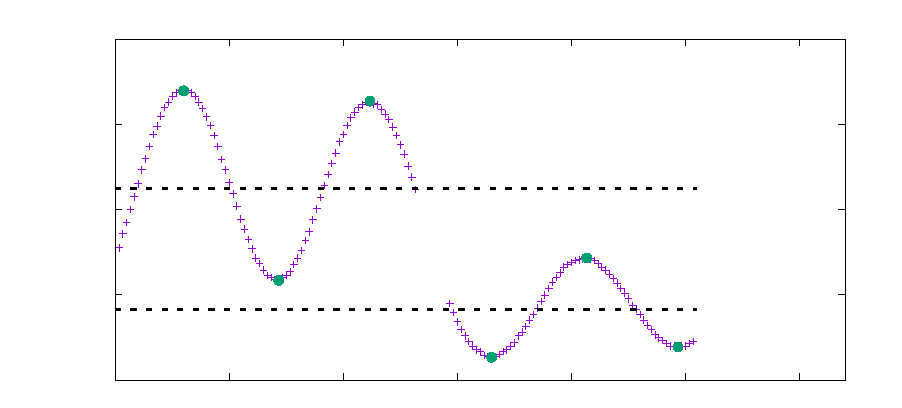
\includegraphics[width={417.60bp},height={180.00bp}]{cavendish}}%
    \gplfronttext
  \end{picture}%
\endgroup

  \caption{Graf závislosti polohy laseru na čase}
\end{figure}

\begin{flalign}
  & \text{poloměr torzního kyvadla } &   d &= 50\ mm & \\
  & \text{vzdálenost bližších dvou koulí } &  r &= 46.5\ mm & \\
  & \text{poloměr kuliček } &  \rho &= 8.19\ mm & \\
  & \text{hmotnost větší wolframové koule } &  M &= 1.5\ kg & \\
  & \text{hmotnost kuličky } &  m &= (38.3 \pm 0.2)\ g & \\
  & \text{perioda kmitů } &  T &= (490 \pm 3)\ s & \\
  & \text{Vzdálenost stínítka od oscilátoru } &  L &= (5.280 \pm 0.003)\ m & \\
  & \text{Dopočítaný rozdíl výchylek} & \varphi_0 - \varphi_0' &= (0.0269 \pm 0.0022)\cdot 10^{-3} \ Rad &
\end{flalign}

Vyjádřením gravitační konstanty ze vztahů (5) (6) a (8) získávám hodnotu

\begin{equation}
  G = (17.4 \pm 1.5) 10^{-11} \text{ Nm}^2 \text{kg}^{-2} \\
\end{equation}

\section{Závěr}

Pomocí reverzního kyvadla jsem změřil gravitační zrychlení v laboratoři $g=(9.800 \pm 0.005) \text{ ms}^{-2}$, která velmi dobře odpovídá tabulkovým hodnotám pro Brno $g=9,809980$ ms$^{-2}$. Na nejistotu má převážně vliv nejistota změřené periody. \\

Gravitační konstantu jsem pomocí Cavendishovy metody určil na $G=17.4 \pm 1.5\cdot 10^{-11}$ Nm$^{2}$kg$^{-2}$ oproti tabulkové hodnotě 6.67430 $\cdot 10^{-11}$ Nm $^{2}$kg$^{-2}$. Na odkaze [1] přikládám článek z Harvardské univerzity, popisující měření stejnou aparaturou jako jsem používal já. Jejich změřená úhlová výchylka, ale byla $0.00540$ Rad, zatímco moje hodnota je $\frac{\varphi_0 - \varphi_0'}{2} = 0.0135$ Rad. Neznám důvod této chyby, ale je příčinou nesprávné hodnoty gravitační konstanty. Periody kmitání máme přibližně shodné. \\


\begin{thebibliography}{0}
\bibitem{tabulky} Cavendishův experiment Harvardské univerzity ~\url{https://sciencedemonstrations.fas.harvard.edu/presentations/cavendish-experiment}.   
\end{thebibliography}

\end{document}

